\chapter{基础知识}
\label{ch2}
我们在本章节中介绍了本文研究所需要的一些基本知识,有助于更好的理解之后章节的内容。

\section{深度神经网络}
深度神经网络基于模块化思想,通过在多个层次上部署多个神经元并通过逐层训练的手段调整神经元间的连接权值,从而实现原始特征数据进行多次非线性变换,对于任何有限给定输入/输出数据的拟合,最终获取到稳定的特征用于后续的问题分析。

神经网络的设计来源于人脑的结构,是人脑处理信息方式的一个简化模型。人类的大脑是人中枢神经系统中的主要部分,这些神经元像网状物一样相互连接。来自外部环境的刺激或来自感觉器官的输入通过感受器之后进入传入神经,神经元一层一层兴奋(激活)后,传导到神经中枢(大脑或脊髓),相当于输出层,神经中枢根据信号的类型做出不同的判断(分类),然后再下达命令,将信号传递到输出神经。不同的信号,大脑都可以进行学习和分辨,而这一通用的模型,就是神经网络。如果你能把几乎任何传感器接入到大脑中,大脑的学习算法就能找出学习数据的方法,并处理这些数据。

如图\ref{fig:深度神经网络结构图}所示,神经网络的基本单元是神经元,由数千甚至数百万个简单的神经元组成,这些神经元密集地相互连接,神经元按层排列。每一层有多个神经元,层与层之间是"前馈传播"的,也就是说,网络中的数据只在一个方向上移动。一个单独的神经元可能与它前面一层的几个神经元相连,它从这些神经元接收数据;与它后面一层的几个神经元相连,它向这些神经元发送数据。神经元之间不存在同层连接,也不存在跨层连接。

\begin{figure}[!hbt]
\centering
	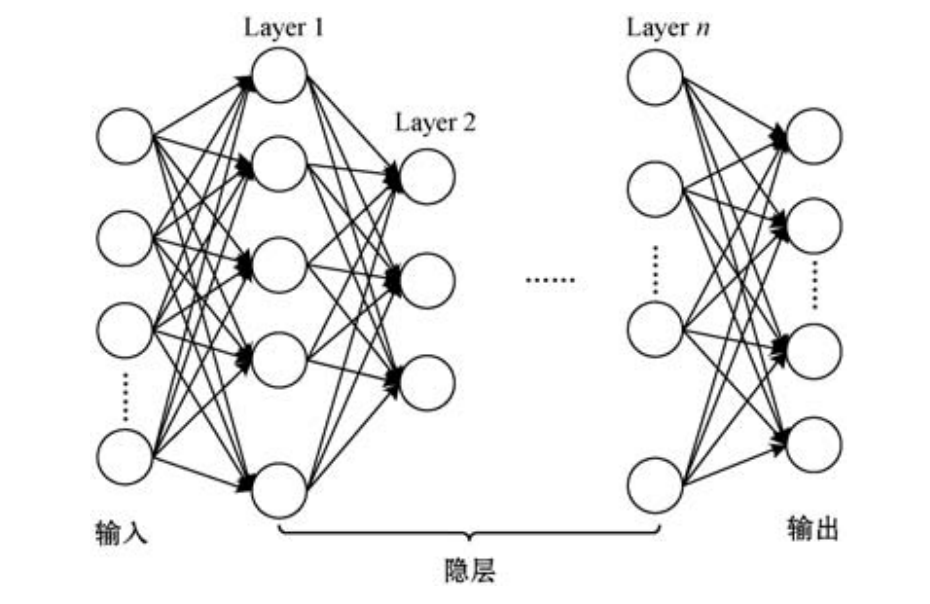
\includegraphics[scale=0.7]{fig2/C2/深度神经网络结构图}%
	\caption{深度神经网络结构图}
	\label{fig:深度神经网络结构图}	
\end{figure}

神经网络通常有三个部分:一个输入层,主要用于获取输入的信息;一个或多个隐藏层,主要进行特征提取,调整权重让隐藏层的神经单元对某种模式形成反应;以及一个输出层,对接隐藏层并输出模型结果,调整权重以对不同的隐藏层神经元刺激形成正确的反应。
当一个神经网络被训练时,其所有的权重和阈值最初都被设置为随机值。训练数据被送入输入层--并通过后续隐藏层,以复杂的方式相乘和相加,直到最后到达输出层,从根本上改变了数据。在训练过程中,不断调整网络的权重和阈值,直到具有相同标签的训练数据持续产生类似的输出。

所谓的前向传播算法就是:将上一层的输出作为下一层的输入,并计算下一层的输出,一直到运算到输出层为止。如图\ref{fig:前馈神经网络结构图}所示,假设现有输入层的训练数据为$D=\left\{\left(x_{1}, y_{1}\right),\left(x_{2}, y_{2}\right), \cdots,\left(x_{m}, y_{m}\right)\right\}, x_{i} \in R^{d}, y_{i} \in R^{l}$,即输入样本由 $d$ 个属性描述, 输出是 $l$ 维实值向量。

\begin{figure}[!hbt]
\centering
	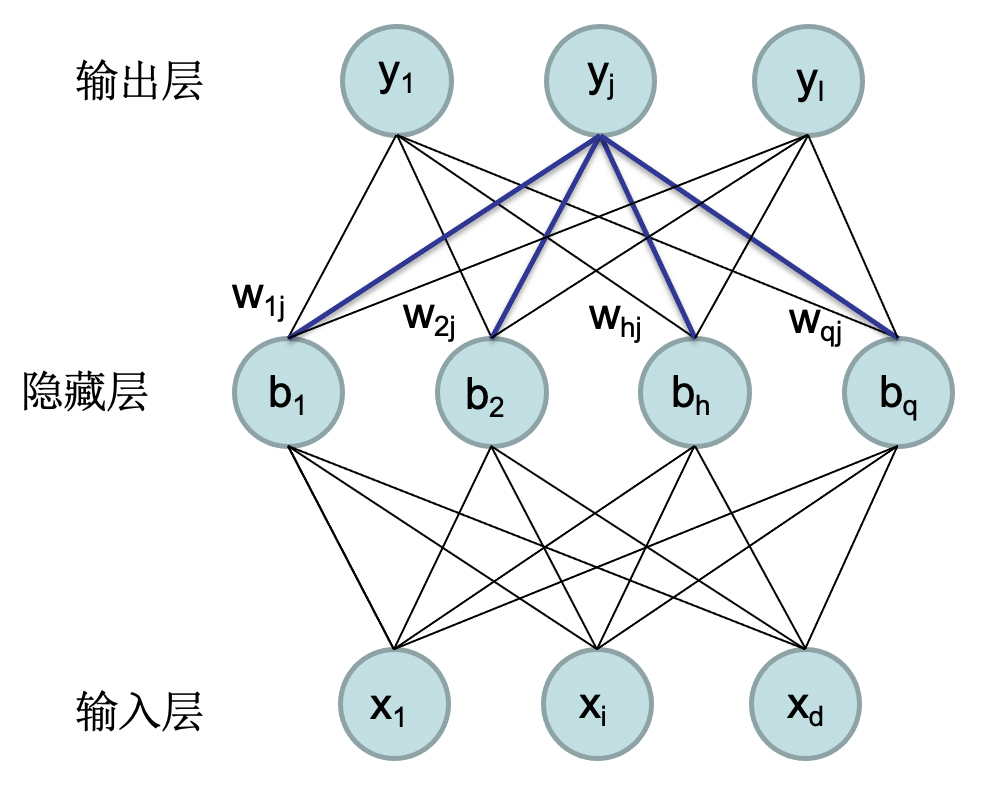
\includegraphics[scale=0.7]{fig2/C2/前馈神经网络}%
	\caption{前馈神经网络结构图}
	\label{fig:前馈神经网络结构图}	
\end{figure}

假设隐藏层神经元个数为$q$个,$\theta_{j}$ 表示输出层神经元的阈值。隐藏层第 $h$ 个神经元的阈值用 $\gamma_{h}$ 表示。
输入层第 $i$ 个神经元与隐藏层第 $h$ 个神经元之间的连接权为 $v_{i h}$。隐藏层第 $h$ 个神经元与输出层第$j$个神经元之间的连接权为 $w_{h j}$ 。
隐藏层第 $h$ 个神经元接收到的输入为$\alpha_{h}=\sum_{i=1}^{d} v_{i h} x_{i}$,输出层第$j$个神经元接收到的输入为$\beta_{j}=\sum_{h=1}^{q} w_{h j} b_{h}$。其中 $b_{n}$ 为隐藏层层第$h$ 个神经元的输 出。
假设隐层和输出层神经元都使用Sigmoid激活函数。对训练例 $\left(x_{k}, y_{k}\right)$, 假定神经网络的输出为 $\hat{y}_{k}=\left(\hat{y}_{1}^{k}, \hat{y}_{2}^{k}, \cdots, \hat{y}_{l}^{k}\right)$, 即神经网络的预测输出表达式为:
\begin{equation}\label{神经网络预测输出}
\hat{y}_{j}^{k}=f\left(\beta_{j}-\theta_{j}\right)
\end{equation}

那么如何评估所提神经网络输出预测值与真实值之间的差异程度呢?这里提出损失函数 $L$ , 文中采用均方差损失函数,表示为:
\begin{equation}\label{神经网络损失函数}
L(\theta,x)=\frac{1}{n} \sum_{i=1}^{n}\left(y_{i}-x_{i}\right)^{2}
\end{equation}

\ref{神经网络损失函数}式中: $\theta$ 为待训练的神经网络权重系数;$x$ 表示目标值;$y$ 表示预测值输出,标 $i$ 表示样本标签。深度神经网络算法训练的目的就是使得损失函数 $L$ 最小。而对于复杂的神经网络而言,最小化损失函数 $L$ 通常采用随机梯度下降( stochastic gradient descent, SGD)算法来完成。即每次迭代过程中随机进行批量抽取训练样本 (记为 $B)$,并计算损失函数 $L$ 的偏导数 $g_{B}=\frac{1}{|B|} \sum_{x \in B} \nabla_{\theta} L(\theta,$,$x$ ),然后沿着负梯度方向 $-g_{B}$ 朝向局部最小值进行更新权重系数 $\theta_{\circ}$。

\section{联邦学习}

\subsection{基本介绍}
深度学习的成功应用需要建立在大量数据的基础之上,才能完成人们指派的学习任务。然而,近年来数据泄漏和隐私侵权事件不断发生,用户开始更加关注他们的隐私信息是否未经自己的许可,或被他人出于商业或者政治目的而被利用。人们逐渐地意识到,在人工智能的构建与使用的过程中保护用户隐私和数据机密的重要性。

大部分拥有的训练数据是由不同组织的个人、部门产生并拥有的,传统机器学习的做法是收集数据并传输到一个中心服务器,服务器可以看见并控制所有的数据,因此这个中心点不仅需要拥有高性能的计算集群来训练和建立机器学习模型,而且还需要处理敏感数据,避免泄漏用户隐私。然而,这种方法需要用户对服务器的完全信任,这已经不再有效或适用了。在这样的情况下,数据拥有者倾向于将自己的数据保留在自己的手中,进而会形成各自孤立的数据孤岛,至此大量数据的基础已经消失,人工智能的未来将面临绝境。作为回应,2016 年谷歌\upcite{ref25}率先提出联邦学习概念,旨在建立高质量分布式学习的框架。在联邦学习系统中,数据所有者(参与者)不需要彼此共享原始数据,也不需要依赖单个可信实体(中心服务器)来进行机器学习模型的分布式训练。相反,参与者通过在自己的本地数据上执行本地训练算法,并且只与参数服务器共享模型参数,来共同协作训练联邦模型。在每轮训练中,参数聚合节点会随机选择合适的节点加入到训练池中。那些被选中的本地节点通常是保持充电且无线网络可用。然后参数聚合节点平均所有已提交者的权重并作为下一轮回合的初始化模型。重复此过程直至终止条件。

根据用户维度和模型特征维度的重合去分类,将联合学习分为水平联邦学习、纵向联邦学习和联合迁移学习\upcite{ref26}。
\begin{itemize}
\item \textbf{水平联邦学习}:当两个数据集的用户属性重叠较多而用户重叠较少的情况下,我们对数据集进行横向切割(即按用户维度切割),取出两边用户属性相同但用户不完全相同的那部分数据用于训练。这种方法被称为横向联合学习。例如,两家银行位于不同的地区,有来自各自地区的用户群,而且它们之间的联系非常少。然而,他们的业务活动非常相似,因此他们的用户特征也是一样的。在这个阶段,我们可以使用跨部门的联合学习来建立一个联合模型。2016年,谷歌提出了一个在安卓手机上更新模型的联合数据建模系统:模型参数在本地不断更新,并在各个用户使用安卓手机时上传到安卓云端,使拥有数据的每一方都能建立一个具有相同特征维度的联合模型。

\item \textbf{纵向联邦学习}:在两个数据集中用户重叠较多,而用户属性重叠较少的情况下,我们将数据集纵向切开(即按特征维度),选择数据集中两边用户相同但用户属性不完全相同的部分进行训练。这种方法被称为纵向的联合学习。例如,有两个不同的组织,一个是在一个地方的银行,另一个是在同一个地方的电子商务公司。他们的用户群很可能包括该地的大部分人口,所以有很大的用户交集。然而,由于银行储存的是用户的收入和支出以及信用评分的数据,而电子商务公司储存的是用户的浏览和购买历史的数据,他们的用户档案并没有那么紧密的联系。长期的联邦学习是在一个加密的空间里将这些不同的功能结合起来,以提高模型的性能。渐渐地,人们发现可以在这个联合系统之上建立若干机器学习模型,如逻辑回归、树状结构和神经网络模型。

\item \textbf{联合迁移学习}:联合迁移学习是通过使用迁移学习模型来弥补数据或标签的差距,而不是对数据进行切分,两个数据集中的用户和用户属性几乎没有重叠。这种方法被称为混合式学习迁移。这里举一个例子,考虑两个不同的组织,一个是中国的银行,另一个是美国的电子商务公司。由于地理上的限制,这两个机构的用户群重叠的地方很少。由于它们是不同类型的组织,数据的特点也没有太多的重叠。在这种情况下,为了保证有效的联邦学习,有必要引入反式学习,以克服单变量数据量小和标注样本小的问题,提高模型的效率。

\end{itemize}

\subsection{模型框架}
本文我们提出的方案是基于典型的分布式横向协作学习系统架构,即各个参与者的本地数据集特征空间相同,但样本不同。通过中心服务器,各个参与者相互协作,在保护个人本地敏感数据的同时,有效地提高本地学习效果。通常这种系统包含以下步骤:

\begin{itemize}
\item 步骤1:中央服务器初始化联合训练模型,然后将初始参数传递给每一个本地客户端。
\item 步骤2:客户端在本地数据上使用中央服务器传递的模型参数进行模型训练。
\item 步骤3:中央服务器汇总此次通信回合中所有参与者上传的模型参数,并对其进行聚合求得全局模型的参数,然后更新全局模型。
\item 步骤4:客户端更新各自的本地模型,重复步骤2-4直至中心服务器的联合模型收敛。
\end{itemize}


\section{差分隐私}
差分隐私作为一种隐私保护方法是为一个用户服务的,因为根据隐私的定义,隐私泄露只是与特定用户有关的信息泄露,而一组用户的统计特征不包括在隐私信息中。如果一个对象在数据库中的存在或不存在,或其价值的变化不会对搜索结果产生重大影响,那么该对象的隐私信息就会受到保护,这就是差分隐私(DP)概念的起源。差分隐私首先被应用于数据查询,为了更好地说明数据集之间的差异,定义了相邻数据集的概念:两个数据集只差一个信息或只差一个数值不同的记录\upcite{ref28}。因此,查询数据库相关信息的攻击者将无法以任何概率确定$X_{n}$是否存在于数据集中,而成员$X_{n}$被认为是相对安全的。


\subsection{基本定义}
对于一个有限域 $Z, z \in Z$ 为 $Z$ 中的元素, 从 $Z$ 中抽样所得 $z$ 的集合组成数据集 $D$, 其样本量为 $n$, 属性的个数为维度 $d$。对数据集 $D$ 的各种映射函数被定义为查询 (Query), 用 $F=\left\{f_{1}, f_{2}, \cdots\right\}$ 来表示一组查询,算法 $M$ 对查询 $F$ 的结果进行处理,使之满足隐私保护的 条件,此过程称为隐私保护机制。设数据集 $D$ 和 $D^{\prime}$,具有相同的属性结构,两者 的对称差记作 $D \Delta D^{\prime},\left|D \Delta D^{\prime}\right|$ 表示 $D \Delta D^{\prime}$ 中记录的 数量。若 $\left|D \Delta D^{\prime}\right|=1$, 则称 $D$ 和 $D^{\prime}$ 为邻近数据集 (Adjacent Dataset)。
\begin{figure}[!hbt]
\centering
	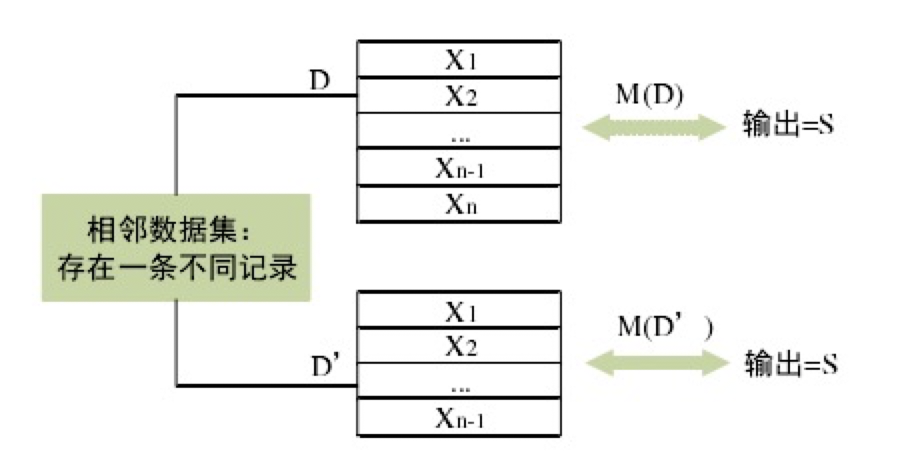
\includegraphics[scale=0.7]{fig2/C2/相邻数据集示意图}%联邦学习的系统架构
	\caption{差分隐私的相邻数据集示意图}
	\label{fig:相邻数据集示意图}	
\end{figure}


\begin{define}[成立条件]\label{成立条件}

若随机算法 $M: D \rightarrow R$ 满足 $(\varepsilon, \delta)-D P$, 当且仅当相邻数据集 $d, d^{\prime}$ 对于算法 $M$ 的所有可能输出子集 $S \in R$ 满足不等式 $^{[40]}$ :
$$
\operatorname{Pr}[M(d) \in S] \leq e^{\varepsilon} \operatorname{Pr}\left[M\left(d^{\prime}\right) \in S\right]+\delta
$$

其中,$\varepsilon$ 表示隐私预算参数, $\varepsilon$ 越小意味着隐私预算越低, 信息泄露越少,隐私保护的强度越高。添加项 $\delta$代表允许以概率 $\delta$ 打破 $\varepsilon-\mathrm{DP}$ 的可能性, 其值通常选择为小于 $1 /|D|$. 当 $\delta=0$ 时, 定义转化为 $\varepsilon-\mathrm{DP}$, 这时机制提供了更加严格的隐私保护。隐私预算参数决定着隐私保护强度, 针对传统数据库保护,当 $\varepsilon \in(0,1)$ 时认为隐私保护强度是有效的, 但 应用在深度学习领域, $\varepsilon \in(0,10)$ 都认为是可以被接受的合理范围。

\end{define}

\subsection{相关概念}
差分隐私保护可以通过在查询函数的返回值中加人适量的干扰噪声来实现。加入噪声过多会影响结果的可用性,过少则无法提供足够的安全保障。敏感度是决定加人噪声量大小的关键参数,它指删除数据集中任一记录对查询结果造成的最大改变。 在差分隐私保护方法中定义了两种敏感度,即全局敏感度(Global Sensitivity)和局部敏感度(Local Sensitivity)。

\begin{define}[全局敏感度]\label{全局敏感度}
设有函数 $f: D \rightarrow R^{d}$, 输人为一数据集,输出为一$d$ 维实数向量。 对于任意的邻近数据集 $D$ 和 $D^{\prime}$,
$$
G S_{f}=\max _{D, D^{\prime}}\left\|f(D)-f\left(D^{\prime}\right)\right\|_{1}
$$
称为函数 $f$ 的全局敏感度。
\end{define}

函数的全局敏感度由函数本身决定,不同的函数会有不同的全局敏感度,一些函数具有较小的全局敏感度(例如计数函数,其全局敏感度为1),因此只需加入少量噪声即可掩盖因一个记录被删除对查询结果所产生的影响,实现差分隐私保护。

\begin{define}[局部敏感度]\label{局部敏感度}
对于一个查询函数 $f_{:} D \rightarrow R^{d}$, 其中 $D$ 为一个数据集, $R^{d}$为d维实数向量,是查询的返回结果。对于给定的数据集D和它的任意邻近数据集 $D^{\prime}$, 有 $f_{\text {在 }} D$ 上的局部敏感度为:
$L S_{f}(D)=\max _{D^{\prime}}\left\|f(D)-f\left(D^{\prime}\right)\right\|_{1}$
\end{define}

局部敏感度由函数及给定数据集中的具体数据共同决定。由于利用了数据集的数据分布特征,局部敏感度通常要比全局敏感度小得多。
敏感度代表了查询函数针对相邻数据集的输出的最大不同,或者说量化评估了最坏情况下单个样本对整体数据带来的不确定性大小。敏感度函数仅与查询函数的类型有关,为扰动的添加提供了依据。但是,由于局部敏感度在一定程度上体现了数据集的数据分布特征,如果直接应用局部敏感度来计算噪声量则会泄露数据集中的敏感信息。

全局差分隐私技术旨在实现这样一个目标:如果替换数据集中的任意样本的效果足够小,则查询结果不能被用来探索数据集中任何样本的更多信息\upcite{ref29}。作为一种优势,这种技术比局部差分隐私技术更准确,因为它不需要向数据集添加大量的噪声。局部差分隐私技术被引入以去除全局差分隐私中所要求的受信任的中央机构\upcite{ref30}。与全局差分隐私技术相比,局部差分隐私技术不需要可信的第三方\upcite{ref31}。其缺点是,噪声总量比全局差分隐私技术大得多。

可量化性、可组合性和后处理不变性是差分隐私最重要的三个性质。可量化性指的是差分隐私算法在计算特定随机化过程时,可以透明化、精准量化所施加的扰动,即上文提及的隐私预算。这样使用者就可以清楚地知道算法的隐私保护力度;组合性可以将相互独立的差分隐私算法进行组合;差分隐私的后处理不变性,确保了即使对算法的结果进行进一步处理,只要不引入额外信息,后处理就并不会削弱算法的隐私
保护力度。 通过组合定理,人们可以利用基础的差分隐私算法设计出复杂的满足差分隐私保证的系统,这也是差分隐私的重要优势之一。 

在差分隐私部署过程中常常不仅仅在一处添加噪声, 也不仅仅针对数据集进隐私预算的分配有序列组合性和并行组合性两种组合特性:

\begin{theorem}[串行组合]\label{串行组合}
给定 $\mathbf{n}$ 个陏机算法 $M_{i}(1 \leq i \leq n)$ 满足 $\varepsilon_{i}-DP$, 那么针对一个数据库 $D$ 而言, 在 $\mathrm{D}$ 上的算法序列组合可以提供 $\varepsilon-\mathrm{DP}$, 其中 $\sum_{i=1}^{n} \varepsilon_{i}=\varepsilon$ 。
\end{theorem}

\begin{theorem}[并行组合]\label{并行组合}
对于数据库 $\mathrm{D}$, 当其被划分成 $\mathrm{n}$ 个不相交的子集 $\left\{\mathrm{D}_{1}, \mathrm{D}_{2}, \ldots, \mathrm{D}_{n}\right\}$, 在每个子集上应用算法 $\mathrm{M}_{i}$, 每个算法提供 $\varepsilon_{i}-\mathrm{DP}$ , 则在序列 $\left\{\mathrm{D}_{1}, \mathrm{D}_{2}, \ldots, \mathrm{D}_{n}\right\}$ 上整体满足 $\left(\max \left\{\varepsilon_{1}, \ldots, \varepsilon_{n}\right\}\right)-\mathrm{DP}$
\end{theorem}


\subsection{实现机制}
在实践中为了使一个算法满足差分隐私保护的要求,对不同的问题有不同的实现方法,这些实现方法称为“机制”。拉普拉斯机制(Lapalace Mechanism)、指数机制(ExponentialMechanism)与高斯机制是三种最基础的差分隐私保护实现机制。其中,Laplace机制和高斯适用于对数值型结果的保护,指数机制则适用于非数值型结果。

在中心化差分隐私中,最为常用的扰动机制是拉普拉斯(Laplace)机制,该机制可以后期处理聚合查询(例如,计数、总和和均值)的结果以使它们差分私有。
Laplace分布是统计学中的概念,是一种连续的概率分布。

\begin{theorem}[拉普拉斯机制]\label{拉普拉斯机制}
如果随机变量的概率密度函数分布为:

$f(x \mid \mu, b)=\frac{1}{2 b} \exp \left(-\frac{|x-\mu|}{b}\right)=\frac{1}{2 b}\left\{\begin{array}{ll}\exp \left(-\frac{\mu-x}{b}\right) & x<\mu \\ \exp \left(-\frac{x-\mu}{b}\right) & x \geq \mu\end{array}\right.$
\end{theorem}

其中,D表示数据集,$f(D)$表示的是查询函数,$Y$表示的是Laplace随机噪声,$M(D)$表示的是最后的返回结果。
$M(D)=f(D)+Y$
如果噪声 $Y \sim L\left(0,\frac{\Delta f}{\longrightarrow}\right)$ 满足 $(\epsilon,0)-$,则表示服从拉普拉斯分布的随机噪声。因此,当隐私预算确定时,敏感度越大,引入的噪声量越大。

对于非数值型的查询结果或数据,通常使用指数机制来随机选择离散的输出结果来满足差分隐私。指数机制整体的思想就是,当接收到一个查询之后,不是确定性的输出一个$R_{i}$结果,而是以一定的概率值返回结果,从而实现差分隐私。而这个概率值则是由打分函数确定,得分高的输出概率高,得分低的输出概率低。

\begin{theorem}[指数机制]\label{指数机制}
指数机制满足差分隐私, 如果:
$$
A(D,u)=\left\{p: \mid \operatorname{Pr}[p \in O] \propto \exp \left(\frac{\varepsilon u(D,p)}{2 \Delta u}\right)\right\}
$$
\end{theorem}
其中 $\Delta u$ 为打分函数 $u(D,p)$ 的全局敏感性。 由式\ref{指数机制}可知, 打分越高被选择输出的概率越大。\upcite{ref53}

与拉普拉斯机制类似高斯机制对输入的所有维度施加高斯噪声干扰 $N\left(0,\sigma^{2}\right)$。
\begin{theorem}[高斯机制]\label{高斯机制}
对于任意 $\varepsilon \in(0,1)$ 与 $c^{2}>2 \ln (1.25 / \delta)$, 参数满足 $\sigma \geq c \Delta_{2} f / \varepsilon$ 的高斯机制为 $(\varepsilon,\delta)$-差分隐私。
\end{theorem}

\section{联邦学习中的差分隐私}
传统的联邦学习中使用差分隐私的主要流程如下所示:
\begin{itemize}
\item 本地计算:
客户端 $\mathrm{i}$ 根据本地数据库 $\mathcal{D}_{\mathrm{i}}$ 和接受的服务器的全局模型 $\mathrm{w}_{\mathrm{G}}^{\mathrm{t}}$ 作为本地的参数,即 $\mathrm{w}_{\mathrm{i}}^{\mathrm{t}}=\mathrm{w}_{\mathrm{G}}^{\mathrm{t}}$, 进 行梯度下降策略进行本地模型训练得到 $\mathrm{w}_{\mathrm{i}}^{\mathrm{t}+1} \quad(\mathrm{t}$ 表示当前round) 。

\item: 模型扰动:
每个客户端产生一个随机噪音 $\mathrm{n},\mathrm{n}$ 是符合高斯分布的,使用 $\overline{\mathbf{w}_{\mathrm{i}}}^{\mathrm{t}+1}=\mathrm{w}_{\mathrm{i}}^{\mathrm{t}+1}+\mathrm{n}$ 扰动本地模型 (这里注意w是一个矩阵,那么n就对矩阵的每一个元素产生噪音)。

\item 模型聚合:
服务器使用FedAVG算法聚合从客户端收到的 $\overline{\mathrm{w}}_{\mathrm{i}} \mathrm{t}+1$ 得到新的全局模型参数 $\mathrm{w}_{\mathrm{G}}^{\mathrm{t}+1}$, 也就是扰动过的 模型参数。

\item 模型广播:
服务器将新的模型参数广播给每个客户端。

\item 本地模型更新:
每个客户端接受新的模型参数,重新进行本地计算。
\end{itemize}

上述的差分隐私技术将原始数据集中到一个数据中心,然后发布满足差分隐私的相关统计信息,我们称其为中心化差分隐私(centralized differential privacy)技术。因此,中心化差分隐私对于敏感信息的保护始终基于一个前提假设:可信的第三方数据收集者,即保证第三方数据收集者不会窃取或泄露用户的敏感信息。然而,在实际应用中,即使第三方数据收集者宣称不会窃取和泄露用户的敏感信息,用户的隐私依旧得不到保障。由此可知,在实际应用中想要找到一个真正可信的第三方数据收集平台十分困难,这极大地限制了中心化差分隐私技术的应用。鉴于此,在不可信第三方数据收集者的场景下,本地化差分隐私(local differential privacy)\upcite{ref32}\upcite{ref33}技术应运而生,其在继承中心化差分隐私技术定量化定义隐私攻击的基础上,细化了对个人敏感信息的保护。具体来说,其将数据的隐私化处理过程转移到每个用户上,使得用户能够单独地处理和保护个人敏感信息,即进行更加彻底的隐私保护。目前,本地化差分技术在工业界已经得到运用:苹果公司将该技术应用在操作系统IOS10上以保护用户的设备数据,谷歌公司同样使用该技术从Chrome浏览器采集用户的行为统计数据\upcite{ref34}。


\section{本章小结}
本章对论文需要使用的一些基础理论知识进行了讨论。主要介绍了联邦学习系统的学习协议以及差分隐私的基本概念、定义和定理,分布式联邦学习系统是本论文主要使用的系统架构,所提的攻击模型和隐私对策都是基于该分布式联邦学习系统。本章同时也介绍了差分隐私及其变体的概念、实现机制。最后介绍了联邦学习中各个神经网络的基本结构和随机梯度下降算法。
